%!TeX root=../ordenacao.tex

\section{Árvore binária de busca balanceada} \label{abb}

Manter um vetor ordenado é uma boa maneira de resolver o problema da
lista ordenada cinética dando suporte às operações
\textsc{advance}$(t)$, \textsc{change}$(j,v)$ e
\textsc{query\_kth}$(i)$. Poderíamos também querer dar suporte, além
das operações citadas, às seguintes operações:
\begin{itemize}
    \item \textsc{insert}$(v, x_t) \rightarrow$ insere um
    elemento com velocidade $v$ e valor $x_t$ no instante \now;
    \item \textsc{delete}$(i) \rightarrow$ remove o elemento
    $i$ no instante \now.
\end{itemize}
Para inserir um elemento no vetor, antes teríamos de encontrar a
posição que este deveria ocupar no vetor. Digamos que seja a
posição $j$. Após encontrar a posição, movemos todos os
elementos, a partir da posição $j$, uma posição à frente e
colocamos o elemento na posição~$j$. Após isso, os certificados
de $j$~até~$n - 1$ devem ser atualizados, pois esses elementos
mudaram de posição no vetor, e um novo certificado será criado,
o $n$-ésimo certificado, o total de elementos $n$ deve ser
mudado para $m = n + 1$. O novo certificado também deve ser
inserido na fila com prioridades.

Essa sequência de operações pode se tornar pouco eficiente com
uma grande quantidade de elementos sendo inseridos no começo do
vetor, consumindo tempo linear por inserção. Como a remoção
envolve uma sequência de operações parecida, da mesma maneira se
torna pouco eficiente, também consumindo tempo linear.

Dessa forma, apesar da lista ordenada cinética implementada
manipulando um vetor ser uma estrutura eficiente para a operação
\textsc{query\_kth}$(i)$, com um consumo de tempo constante,
o consumo de tempo para as operações \textsc{insert}$(v, x_t)$ e
\textsc{delete}$(i)$ é, no pior caso, proporcional ao número de
elementos, o que pode ser ruim para uma grande quantidade de
elementos, inserções e remoções.

Podemos equilibrar o consumo de tempo das operações
\textsc{query\_kth}$(i)$, \textsc{insert}$(v, x_t)$ e
\textsc{delete}$(i)$ em tempo logarítmico no número de elementos,
usando uma ABBB (árvore binária balanceada de busca). Os pontos
serão armazenados na ABBB tendo o seu valor no instante \now~como
chave.

Além da ABBB, para garantirmos a eficiência das
operações \textsc{event}, \textsc{change}, \textsc{insert} e
\textsc{delete}, cada elemento terá um apontador para o seu
predecessor e um apontador para o seu sucessor, formando
uma lista duplamente ligada ordenada pelo valor do elemento
no instante \now. Veja a figura \ref{fig:abb:exemplo}.

\begin{figure}
    \centering
        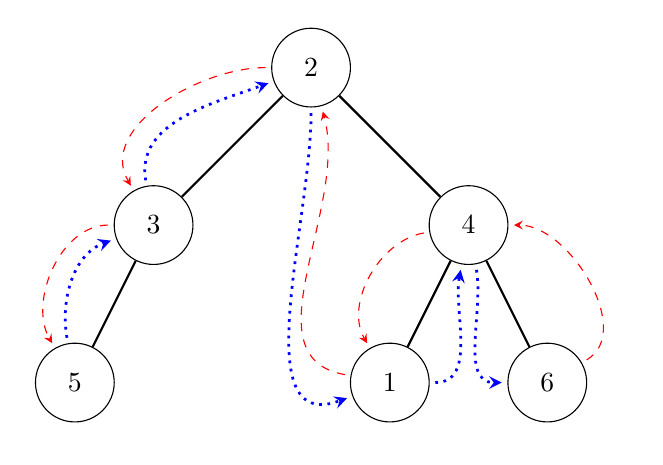
\begin{tikzpicture}[baseline=-2.25cm]
            \node[circle,draw,minimum size=1cm] (1) at (0,0)  {$2$};
            \node[circle,draw,minimum size=1cm] (2) at (-2,-2){$3$};
            \node[circle,draw,minimum size=1cm] (3) at (2,-2) {$4$};
            \node[circle,draw,minimum size=1cm] (4) at (-3,-4){$5$};
            \node[circle,draw,minimum size=1cm] (5) at (1,-4) {$1$};
            \node[circle,draw,minimum size=1cm] (6) at (3,-4) {$6$};
            % \node[label={7},circle,draw,minimum size=1cm] (7) at (3,-4) {$8$};
            % \node[label={8},circle,draw,minimum size=1cm] (8) at (-4,-6) {$4$};
            % \node[label={9},circle,draw,minimum size=1cm] (9) at (-2,-6) {$1$};
            \tikzstyle{filho}=[thick]
            \tikzstyle{pred}=[->, shorten >= 2pt, shorten <= 2pt,
                    dashed, >=stealth, red]
            \tikzstyle{sucessor}=[->, shorten >= 2pt, shorten <= 2pt,
                    dotted, >=stealth, blue, line width=0.35mm]
            % \tikzstyle{p4}=[->, shorten >= 2pt, shorten <= 2pt, dotted, >=stealth]
            \draw[filho] (1) -- (2);
            \draw[filho] (1) -- (3);
            \draw[filho] (2) -- (4);
            \draw[filho] (3) -- (5);
            \draw[filho] (3) -- (6);
            \draw[pred] (6) edge[out=30,in=0] (3);
            \draw[sucessor] (3) edge[out=280,in=180] (6);
            \draw[pred] (3) edge[out=190,in=120] (5);
            \draw[sucessor] (5) edge[out=0,in=260] (3);
            \draw[pred] (5) edge[out=170,in=285] (1);
            \draw[sucessor] (1) edge[out=270,in=200] (5);
            \draw[pred] (1) edge[out=180,in=120] (2);
            \draw[sucessor] (2) edge[out=100,in=200] (1);
            \draw[pred] (2) edge[out=180,in=120] (4);
            \draw[sucessor] (4) edge[out=100,in=200] (2);
        \end{tikzpicture}
        \qquad
        \qquad
        \qquad
        \begin{tabular}{|c|c|}
            \hline
            $i$ & $x_0$ \\
            \hline
            $1$ & $6$ \\

            $2$ & $3$ \\

            $3$ & $2$ \\

            $4$ & $7$ \\

            $5$ & $-2$ \\

            $6$ & $14$ \\
            \hline
        \end{tabular}
        \caption[Exemplo de estrutura da ABB]{Exemplo de árvore em
            que a ordem dos elementos, do menor para o maior no
            instante $\now = 0$, é $5 - 3 - 2 - 1 - 4 - 6$. Os
            apontadores para o elemento anterior são representados
            pelas setas vermelhas tracejadas e os apontadores para o
            elemento posterior são representados pelas setas azuis
            pontilhadas.}\label{fig:abb:exemplo}
\end{figure}

No que diz respeito aos certificados, antes um certificado estava
associado a uma posição e, no vetor, ao inserirmos um elemento em
uma determinada posição, teríamos que deslocar % que atualizar
todos os certificados conseguintes àquela posição. Agora, para que
consigamos alterar apenas uma quantidade constante de certificados
após uma inserção, os certificados não estarão mais associados a uma
posição e sim aos elementos.

O certificado $i$ se refere à relação estabelecida entre o elemento
$i$ e seu predecessor e consiste no instante de tempo em que o
elemento $i$ deixará de ter um valor maior que o valor do seu
predecessor, se esse instante for maior que o instante atual. Do
contrário, o certificado consiste em $+\infty$. Se o elemento $i$
não possui predecessor, então o certificado também consiste em
$+\infty$. Veja a Figura \ref{fig:abb:cert}.

Esses $n$ certificados também serão colocados em uma fila com
prioridades, com o prazo de validade determinando a prioridade.
A fila com prioridades agora também deverá suportar operações
como a inserção e remoção de certificados.

\begin{figure}
    \centering
    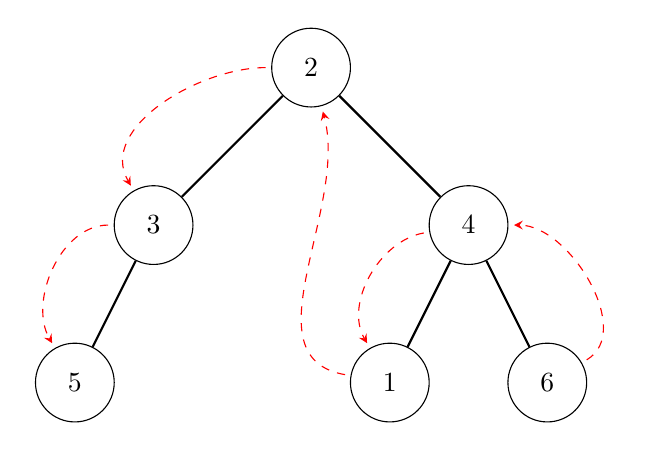
\begin{tikzpicture}[baseline=-2.25cm]
        \node[circle,draw,minimum size=1cm] (1) at (0,0)  {$2$};
        \node[circle,draw,minimum size=1cm] (2) at (-2,-2){$3$};
        \node[circle,draw,minimum size=1cm] (3) at (2,-2) {$4$};
        \node[circle,draw,minimum size=1cm] (4) at (-3,-4){$5$};
        \node[circle,draw,minimum size=1cm] (5) at (1,-4) {$1$};
        \node[circle,draw,minimum size=1cm] (6) at (3,-4) {$6$};
        \tikzstyle{filho}=[thick]
        \tikzstyle{pred}=[->, shorten >= 2pt, shorten <= 2pt,
            dashed, >=stealth, red]
        \tikzstyle{sucessor}=[->, shorten >= 2pt, shorten <= 2pt,
            dotted, >=stealth, line width=0.35mm]
        \draw[filho] (1) -- (2);
        \draw[filho] (1) -- (3);
        \draw[filho] (2) -- (4);
        \draw[filho] (3) -- (5);
        \draw[filho] (3) -- (6);
        \draw[pred] (6) edge[out=30,in=0] (3);
        \draw[pred] (3) edge[out=190,in=120] (5);
        \draw[pred] (5) edge[out=170,in=285] (1);
        \draw[pred] (1) edge[out=180,in=120] (2);
        \draw[pred] (2) edge[out=180,in=120] (4);
    \end{tikzpicture}
    \qquad
    \qquad
    \qquad
    \begin{tabular}{|c|c|c|c|}
        \hline
        $i$ & $x_0$ & $v$ & $\cert[i]$ \\
        \hline
        $1$ & $6$ & $2$ & $1$ \\

        $2$ & $3$ & $5$ & $+\infty$ \\

        $3$ & $2$ & $1$ & $2$ \\

        $4$ & $7$ & $4$ & $+\infty$ \\

        $5$ & $-2$ & $3$ & $+\infty$ \\

        $6$ & $14$ & $0.5$ & $2$ \\
        \hline
    \end{tabular}
    \caption[Representação dos certificados da ABB]{Certificados
            representados pelas setas vermelhas tracejadas. O
            certificado do elemento $5$ vale $+\infty$.}
            \label{fig:abb:cert}
\end{figure}

Para descrever as implementações das operações, vamos
estabelecer os nomes dos objetos, variáveis e rotinas
auxiliares utilizados:
\begin{enumerate}
    \item $n$: número de elementos no instante \now;
    \item \no: objeto que compõe a árvore binária balanceada
            de busca, com atributos:
    \begin{enumerate}
        \item \esq$:$ aponta para a raiz da subárvore
                    esquerda do nó;
        \item \dir$:$ aponta para a raiz da subárvore
                    direita do nó;
        \item \textit{key}$:$ aponta para um elemento;
        \item \children$:$ quantidade de nós que a subárvore
                            deste nó possui.
                        Este atributo será importante para a
                        operação \textsc{query\_kth}$(i)$;
    \end{enumerate}
    \item \raiz: nó que é a raiz da árvore binária balanceada de
                busca;
    \item \elemento: objeto com os seguintes atributos:
    \begin{enumerate}
        \item \id: vem de \textit{identifier} e é o atributo
                    para identificar o objeto. Assim, daqui
                    em diante, usaremos elemento $i$ para nos
                    referirmos ao elemento cujo \id~é $i$;
        \item \speed: velocidade do elemento;
        \item \initv: valor que o elemento possuía no
        instante~$t = 0$;
        \item \nex: atributo que aponta para o elemento
                    imediatamente posterior a este na coleção,
                    no instante \now. O elemento imediatamente
                    posterior a $i$ é aquele que possui o menor
                    valor dentre a coleção de elementos que
                    possuem valor maior que o elemento $i$;
        \item \prev: vem de \textit{previous} e é o atributo
                    que aponta para o elemento imediatamente anterior
                    a este na coleção, no instante \now;
        \item \pqpos: vem de \textit{priority queue position} e
                    é o atributo que aponta para a posição do
                    certificado associado ao elemento na
                    fila com prioridades;
        \item \cert: vem de \textit{certificate} e é o tempo
                    de validade do certificado entre este elemento
                    e o elemento apontado por \prev; se \prev~não
                    aponta para ninguém, \cert~vale $+\infty$;
        \item \no: aponta para o nó da árvore binária de busca
                    em que o elemento se encontra;
    \end{enumerate}
    \item \Q: fila com prioridades que contém os elementos;
            o elemento com certificado de menor valor estará
            à frente da fila;
    \item \textsc{insertKey}$(\text{\raiz},e)\rightarrow$ insere $e$,
                        um elemento, na árvore binária balanceada
                        de busca com raiz \raiz~e retorna a,
                        possivelmente nova, raiz da árvore.
                        No processo também atualiza a lista ligada
                        de elementos;
    \item \textsc{deleteKey}$(\text{\raiz},e)\rightarrow$ remove $e$,
                        um elemento, da árvore binária balanceada
                        de busca com raiz \raiz~e retorna a,
                        possivelmente nova, raiz da árvore.
                        No processo também atualiza a lista ligada
                        de elementos.
\end{enumerate}
Para a implementação das operações \textsc{change}$(j, v)$ e
\textsc{delete}$(i)$, precisamos de alguma maneira recuperar
um elemento baseado no seu \id. Para tal, podemos utilizar
uma tabela de símbolos, implementada por
uma árvore binária balanceada de busca ou uma
tabela de dispersão. A seguir~estão três operações que nos
ajudarão a recuperar os elementos:
\begin{enumerate}
    \item \textsc{getObject}$(i)\rightarrow$ retorna o
    elemento $i$;
    \item \textsc{insertObject}$(e) \rightarrow$ insere $e$,
    que é um elemento, na estrutura;
    \item \textsc{deleteObject}$(e) \rightarrow$ remove $e$,
    que é um elemento, da estrutura.
\end{enumerate}
Para permitir a inserção e remoção de certificados, a
interface da fila com prioridades será reformulada,
contando com duas operações extras:
\begin{enumerate}
    \item \textsc{insertPQ}$(Q, e) \rightarrow$ insere $(e, t)$
    na fila com prioridades $Q$;
    \item \textsc{deletePQ}$(Q, e) \rightarrow$ remove $e$
    da fila com prioridades $Q$;
    \item \textsc{updatePQ}$(Q,e,t) \rightarrow$ muda o
    valor do certificado de $e$ para $t$ e atualiza a fila
    com prioridades $Q$;
    \item \textsc{minPQ}$(Q) \rightarrow$ devolve o elemento
    com o certificado de menor valor da fila com prioridades $Q$.
\end{enumerate}
A operação \textsc{updatePQ}$(Q,e,t)$ pode ser
implementada em tempo logarítmico graças ao atributo
\pqpos~dos elementos.

Um evento está associado a um certificado $(e, t)$ que
expira no instante $t$. O tratamento do evento correspondente
ao certificado $(e, t)$ consiste em trocar de lugar o
elemento $e$ e seu predecessor, digamos $e'$, na
árvore binária de busca e na lista ligada, e
recalcular o prazo de validade de até 3 certificados:
\begin{itemize}
    \item O certificado de $e$;
    \item O certificado de $e'$;
    \item O certificado do novo sucessor de $e'$.
\end{itemize}

Na implementação da operação \textsc{event}, Algoritmo
\ref{abb:evento}, utilizaremos a rotina \textsc{update}$(e)$ que
calcula a nova validade $t$ do certificado do elemento $e$, e chama
a rotina \textsc{updatePQ}$(Q, e, t)$. A função \textsc{swap}$(e_1,
e_2)$ troca a posição de $e_1$ e $e_2$ na árvore binária balanceada
de busca e na lista ligada.

\begin{algorithm}[H]
    \caption{Função \textsc{update}.} \label{torneioi:update}
    \begin{algorithmic}[1]
        \Function{update}{$e$}
            \If{$e \neq$ NULL}
                \State $e'\leftarrow \torneio[(e.\lastmatch)/2]$
                \State $t \leftarrow $ \Call{expire}{$e, e'$}
                \State \Call{updatePQ}{$Q,e,t$}
            \EndIf
        \EndFunction
        % \LineComment{Em expire$(e, e')$, $e'$ pode ser nulo e
        % nesse caso o retorno é $+\infty$.}
        % \LineComment{\Call{expire}{$e,e'$} calcula a validade do
        % certificado entre os elementos $e$ e $e'$, se $e'$ é NULL
        % retorna $+\infty$}
    \end{algorithmic}
\end{algorithm}

\begin{algorithm}[H]
    \caption{Função \textsc{event}.} \label{torneioi:evento}
    \begin{algorithmic}[1]
        \Function{event}{\nnull}
            \State $e \leftarrow  $ \Call{minPQ}{$Q$}
            \While{$e.\cert$ = \now}
                \State $j \leftarrow e.\lastmatch$
                \State $k \leftarrow 2\cdot \floor{\frac{j}{2}}
                + ((j + 1)\mod2)$ \Comment{adversário}
                \While{$j > 1$ \AND \Call{value}{$j$} $\geq$
                    \Call{value}{$k$}}
                    \State \torneio[$\floor{\frac{j}{2}}$]
                    $\leftarrow~$\torneio[$j$]
                    \State $\torneio[k].\lastmatch$ $\leftarrow k$
                    \State \Call{update}{$\torneio[k]$}
                    \State $j \leftarrow \floor{\frac{j}{2}}$
                    \State $k \leftarrow 2\cdot \floor{\frac{j}{2}}
                    + ((j + 1)\mod2)$ \Comment{adversário}
                \EndWhile
                \State $\torneio[j].\lastmatch \leftarrow j$
                \State \Call{update}{$\torneio[j]$}
                \State $e \leftarrow  $ \Call{minPQ}{$Q$}
            \EndWhile
        % \LineComment{swapHeap$(i, \floor{\frac{i}{2}})$ troca \heap[$i$] por \heap$\left[\floor{\frac{i}{2}}\right]$}
        \EndFunction
%        \LineComment{\Call{compare}{$i, j$} retorna se o valor
%        de $i$ é maior que o valor de $j$.}
    \end{algorithmic}
\end{algorithm}

\begin{figure}[H]
    \centering
    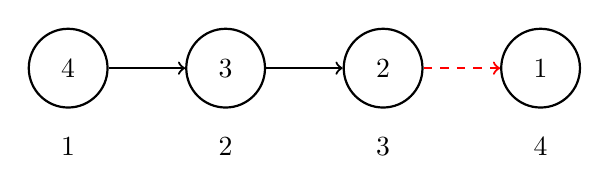
\begin{tikzpicture}[thick]
        \edef\pos{0}
        \foreach \x in {1, 2,..., 4}{
            \pgfmathparse{\pos+2}
            \xdef\pos{\pgfmathresult}
            \node  at (\pos, -1) {$\x$};
        }
        \node[circle,draw, minimum size=1cm] (1) at  (2, 0) {$4$};
        \node[circle,draw, minimum size=1cm] (2) at  (4, 0) {$3$};
        \node[circle,draw, minimum size=1cm] (3) at  (6, 0) {$2$};
        \node[circle,draw, minimum size=1cm] (4) at  (8, 0) {$1$};
        \draw[->] (1) -- (2);
        \draw[->] (2) -- (3);
        \draw[->, color=red, dashed] (3) -- (4);
    \end{tikzpicture}
    \caption[Exemplo de expiração de certificado da lista ordenada]{No exemplo da
    Figura~\ref{fig:ordenacao:exemplo}, \cert[3] expirou no instante $t = 2$.}
    \label{fig:lista:expire}
\end{figure}

\begin{figure}
    \centering
    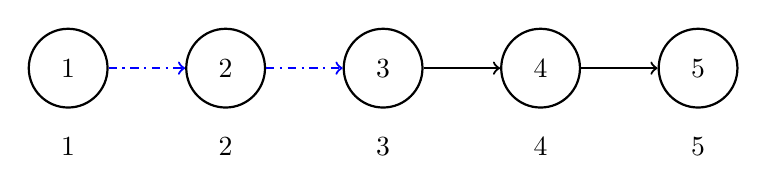
\begin{tikzpicture}[thick]
        \edef\pos{0}
        \foreach \x in {1, 2,..., 5}{
            \pgfmathparse{\pos+2}
            \xdef\pos{\pgfmathresult}
            \node[circle,draw, minimum size=1cm] (\x) at
                (\pos, 0) {$\x$};
            \node  at (\pos, -1) {$\x$};
        }
        % \foreach \x [evaluate=\x as \y using int(\x + 1)] in {1, 2,..., 4}{
        %     \ifthenelse{\x==2}{\draw[->, draw=red] (\x) -- (\y);}{\draw[->, draw=black] (\x) -- (\y);}
        % }
        \draw[->, color=blue, dashdotted] (1) -- (2);
        \draw[->, color=blue, dashdotted] (2) -- (3);
        \draw[->] (3) -- (4);
        \draw[->] (4) -- (5);
        % \draw[->] (1) edge (2) (2) edge (3) (3) edge (4) (4) edge (5)
    \end{tikzpicture}
    \caption[Certificados atualizados]{Após a mudança de velocidade
            do elemento 2, que se encontra em \sorted[2], \cert[1] e
            \cert[2] foram atualizados.}
    \label{fig:lista:after}
\end{figure}

A operação \textsc{query\_kth}$(i)$ consiste em devolver o $i$-ésimo
maior elemento da lista ligada. Para tal, usaremos a árvore binária
balanceada de busca. Estando em um determinado nó \no~da árvore,
sabemos que todos os nós na subárvore direita tem valor maior que o
nó atual e que os nós da subárvore esquerda. Portanto, se $i \leq
node.right.\children$, a nossa resposta com certeza está na
subárvore direita do nó. Caso contrário temos duas opções: \no~é a
resposta ou a resposta está na subárvore esquerda. Para checar se
\no~é a resposta devemos perceber que \no~tem valor maior que os nós
de sua subárvore esquerda, então se $i = node.right.\children + 1$,
\no~é a resposta. Se $i > node.right.\children + 1$, então a nossa
resposta está na subárvore esquerda e queremos o $[i -
(node.right.\children + 1)]-$ésimo elemento da subárvore esquerda.
Podemos repetir esse processo até encontrar a nossa resposta. O
algoritmo \ref{abb:query} utiliza a rotina auxiliar
\textsc{rsize}$(r)$, que devolve o valor de \textit{size} de
$r.right$ caso este seja não nulo, caso contrário devolve $0$.
% Se, dada uma raiz, soubermos a quantidade de filhos direitos,~\raiz$.rsize$, comparamos com o valor de $i$ e podemos ter três conclusões: se~$i > root.rsize$, significa que o $i$-ésimo elemento com certeza não está na subárvore direita, pois todos elementos da subárvore direita estão a frente de \raiz~e da subárvore esquerda. Nesse caso, calculamos $i - root.rsize$, se esse valor é igual a $1$, então \raiz~é o $i-ésimo$ elemento da coleção, pois \raiz~é o próximo elemento após todos elementos na subárvore direita. Se $root.rsize - i \neq 1$, então devemos

\begin{algorithm}
    \caption{Função \textsc{query\_kth}.} \label{abb:query}
\begin{algorithmic}[1]
    \Function{query\_kth}{$i$}
        \State $node \leftarrow root$
        \State $r \leftarrow \Call{rsize}{node}$
        \While{$i \neq r + 1$}
        \If{$i \leq r$}
            \State $node \leftarrow node.right$
        \Else
            \State $node \leftarrow node.left$
            \State $i \leftarrow i - (r + 1)$
        \EndIf
        \State $r \leftarrow \Call{rsize}{node}$
        \EndWhile
        \State \Return $node.key$
    \EndFunction
\end{algorithmic}
\end{algorithm}

\begin{figure}
    \centering
    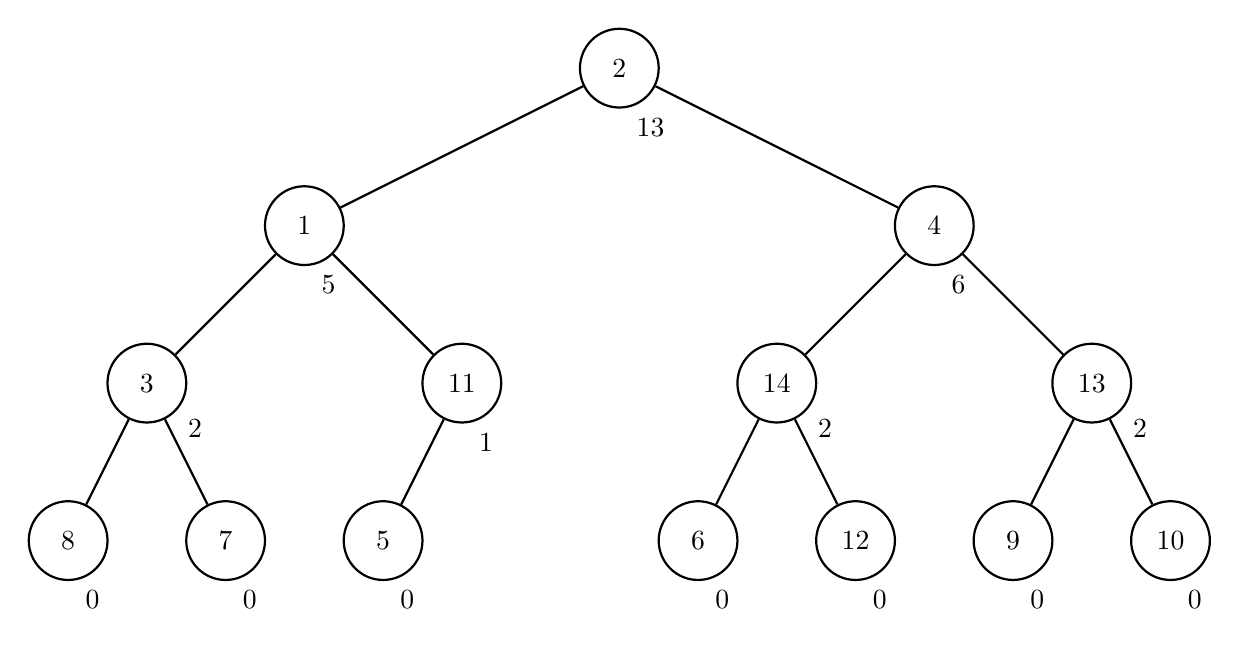
\begin{tikzpicture}[thick]
        \node[label=280:{13},circle,draw,minimum size=1cm]
            (1) at (0,0) {$2$};
        \node[label=280:{5},circle,draw,minimum size=1cm]
            (2) at (-4,-2) {$1$};
        \node[label=280:{6},circle,draw,minimum size=1cm]
            (3) at (4,-2) {$4$};
        \node[label=320:{2},circle,draw,minimum size=1cm]
            (4) at (-6,-4) {$3$};
        \node[label=280:{1},circle,draw,minimum size=1cm]
            (5) at (-2,-4) {$11$};
        \node[label=320:{2},circle,draw,minimum size=1cm]
            (6) at (2,-4) {$14$};
        \node[label=320:{2},circle,draw,minimum size=1cm]
            (7) at (6,-4) {$13$};
        \node[label=280:{0},circle,draw,minimum size=1cm]
            (8) at (-7,-6) {$8$};
        \node[label=280:{0},circle,draw,minimum size=1cm]
            (9) at (-5,-6) {$7$};
        \node[label=280:{0},circle,draw,minimum size=1cm]
            (10) at (-3,-6) {$5$};
        % \node[label={11},circle,draw,minimum size=1cm] (11) at (-1,-6) {$3$};
        \node[label=280:{0},circle,draw,minimum size=1cm]
            (12) at (1,-6) {$6$};
        \node[label=280:{0},circle,draw,minimum size=1cm]
            (13) at (3,-6) {$12$};
        \node[label=280:{0},circle,draw,minimum size=1cm]
            (14) at (5,-6) {$9$};
        \node[label=280:{0},circle,draw,minimum size=1cm]
            (15) at (7,-6) {$10$};

        \draw[thick] (1) -- (2);
        \draw[thick] (2) -- (4);
        \draw[thick] (4) -- (8);
        \draw[thick] (4) -- (9);
        \draw[thick] (2) -- (5);
        \draw[thick] (5) -- (10);
        % \draw[thick] (5) -- (11);
        \draw[thick] (1) -- (3);
        \draw[thick] (3) -- (6);
        \draw[thick] (3) -- (7);
        \draw[thick] (6) -- (12);
        \draw[thick] (6) -- (13);
        \draw[thick] (7) -- (14);
        \draw[thick] (7) -- (15);
    \end{tikzpicture}
    \caption[Como buscar $i$-ésimo na ABB]{Se quiséssemos encontrar
            o $7^\circ$ elemento na árvore acima, $i = 7$, desviamos
            para a direita, pois a quantidade de nós da subárvore
            direita da raiz é $\leq i$. Depois, desviamos para a
            esquerda e redefinimos $i$ como $3$, pois existem $4$
            elementos à frente. Como o nó do elemento $14$ só tem um
            nó em sua subárvore direita, desviamos para a esquerda
            de novo e redefinimos $i$ como $1$. Como a quantidade de
            nós da subárvore direita do nó do elemento $6$  somada a
            $1$ é igual a $i$, o elemento $6$ é o $7^\circ$ elemento
            da coleção.}
    \label{fig:abb:query}
\end{figure}

A operação \textsc{change}$(j, v)$ consiste em recuperar o
elemento $e$ com identificador $j$, alterar seu atributo
\initv~para $x_0 + (\mathit{speed} - v)\cdot now$,
\textit{speed} para \textit{v} e recalcular os eventuais
certificados de que $j$ participa, que seriam $e.cert$ e
$e.next.cert$, se $e.next$ existe.

\begin{algorithm}
    \caption{Função \textsc{change}.} \label{lista:change}
\begin{algorithmic}[1]
    \Function{change}{$j, v$}
        \State $x_0$[$j$] $\leftarrow  x_0$[$j$]
        $+~($\speed[$j$]$~-~v)~\cdot~$\now;
        \State \speed[$j$] $\leftarrow  v$
        \State $i \leftarrow$ \inds[$j$]
        \State \Call{update}{$i$}
        \State \Call{update}{$i - 1$}
    \EndFunction
\end{algorithmic}
\end{algorithm}

\begin{algorithm}
    \caption{Função \textsc{change}.} \label{lista:change}
\begin{algorithmic}[1]
    \Function{change}{$j, v$}
        \State $x_0$[$j$] $\leftarrow  x_0$[$j$]
        $+~($\speed[$j$]$~-~v)~\cdot~$\now;
        \State \speed[$j$] $\leftarrow  v$
        \State $i \leftarrow$ \inds[$j$]
        \State \Call{update}{$i$}
        \State \Call{update}{$i - 1$}
    \EndFunction
\end{algorithmic}
\end{algorithm}

\begin{algorithm}
    \caption{Função \textsc{insert}.} \label{torneioi:insert}
    \begin{algorithmic}[1]
        \Function{insert}{$v, x_t$}
            \State $e.speed \leftarrow v$
            \State $e.x_0 \leftarrow x_t - now\cdot v$
            \State \raiz~$\leftarrow$ \Call{insertObject}{$root, e$}
            \State \Call{insertTourn}{$e$}
            \State \Call{newCert}{$e$}
            \State \Call{insertPQ}{$Q, e$}
        \EndFunction
    \end{algorithmic}
\end{algorithm}

A operação \textsc{insert}$(v, x_t)$ consiste em criar um novo
elemento, inicializando seus atributos com os devidos valores,
inseri-lo na árvore binária balanceada de busca e na estrutura
que usamos para recuperá-lo depois, calcular o seu certificado
e inseri-lo na fila com prioridades e, por fim, atualizar o
certificado de seu sucessor, caso exista. Uma importante o
bservação é que se \now~$\neq 0$, então $x_t \neq$~\initv.
Para calcular \initv, podemos utilizar a relação $x_t = now\cdot
speed + x_0 \Rightarrow x_0 = x_t - speed\cdot now$.

\begin{algorithm}
    \caption{Função \textsc{insert}.} \label{torneioi:insert}
    \begin{algorithmic}[1]
        \Function{insert}{$v, x_t$}
            \State $e.speed \leftarrow v$
            \State $e.x_0 \leftarrow x_t - now\cdot v$
            \State \raiz~$\leftarrow$ \Call{insertObject}{$root, e$}
            \State \Call{insertTourn}{$e$}
            \State \Call{newCert}{$e$}
            \State \Call{insertPQ}{$Q, e$}
        \EndFunction
    \end{algorithmic}
\end{algorithm}

\begin{algorithm}
    \caption[Algoritmo \textsc{delete} da árvore binária de busca]{Função \textsc{delete}.} \label{alg:abb:delete}
    \begin{algorithmic}[1]
        \Function{delete}{$i$}
            \State $e \leftarrow$ \Call{getObject}{$i$}
            \State $e' \leftarrow e.next$
            \State \raiz~$\leftarrow$ \Call{deleteKey}{$\raiz, e$}
            \State \Call{deleteObject}{$e$}
            \State \Call{deletePQ}{$Q, e$}
            \State \Call{update}{$e'$}
        \EndFunction
    \end{algorithmic}
\end{algorithm}

A operação \textsc{delete}$(i)$ consiste em recuperar o elemento
$i$, removê-lo da árvore binária balanceada de busca e da estrutura
que usamos para recuperá-lo, e depois removê-lo da fila com
prioridades. Após isso, basta atualizar o certificado de seu
sucessor, caso exista.

\begin{algorithm}
    \caption[Algoritmo \textsc{delete} da árvore binária de busca]{Função \textsc{delete}.} \label{alg:abb:delete}
    \begin{algorithmic}[1]
        \Function{delete}{$i$}
            \State $e \leftarrow$ \Call{getObject}{$i$}
            \State $e' \leftarrow e.next$
            \State \raiz~$\leftarrow$ \Call{deleteKey}{$\raiz, e$}
            \State \Call{deleteObject}{$e$}
            \State \Call{deletePQ}{$Q, e$}
            \State \Call{update}{$e'$}
        \EndFunction
    \end{algorithmic}
\end{algorithm}
